% Use this template to write your solutions to COS 423 problem sets

\documentclass[12pt]{article}
\usepackage[utf8]{inputenc}
\usepackage{amsmath, amsfonts, amsthm, amssymb, algorithm, graphicx, mathtools, xfrac}
\usepackage[noend]{algpseudocode}
\usepackage{fancyhdr, lastpage}
\usepackage{booktabs}
\usepackage{multirow}
\usepackage{graphicx}
\usepackage{pgfplots}
\usepackage[vmargin=1.20in,hmargin=1.25in,centering,letterpaper]{geometry}
\setlength{\headsep}{.50in}
\setlength{\headheight}{15pt}

% Landau notation
\DeclareMathOperator{\BigOm}{\mathcal{O}}
\newcommand{\BigOh}[1]{\BigOm\left({#1}\right)}
\DeclareMathOperator{\BigTm}{\Theta}
\newcommand{\BigTheta}[1]{\BigTm\left({#1}\right)}
\DeclareMathOperator{\BigWm}{\Omega}
\newcommand{\BigOmega}[1]{\BigWm\left({#1}\right)}
\DeclareMathOperator{\LittleOm}{\mathrm{o}}
\newcommand{\LittleOh}[1]{\LittleOm\left({#1}\right)}
\DeclareMathOperator{\LittleWm}{\omega}
\newcommand{\LittleOmega}[1]{\LittleWm\left({#1}\right)}

% argmin and argmax
\newcommand{\argmin}{\operatornamewithlimits{argmin}}
\newcommand{\argmax}{\operatornamewithlimits{argmax}}

\newcommand{\calP}{\mathcal{P}}
\newcommand{\Z}{\mathbb{Z}}
\newcommand{\R}{\mathbb{R}}
\newcommand{\Exp}{\mathbb{E}}
\newcommand{\Q}{\mathbb{Q}}
\newcommand{\sign}{\mathrm{sign\ }}
\newcommand{\abs}{\mathrm{abs\ }}
\newcommand{\eps}{\varepsilon}
\newcommand{\zo}{\{0, 1\}}
\newcommand{\SAT}{\mathit{SAT}}
\renewcommand{\P}{\mathbf{P}}
\newcommand{\NP}{\mathbf{NP}}
\newcommand{\coNP}{\co{NP}}
\newcommand{\co}[1]{\mathbf{co#1}}
\renewcommand{\Pr}{\mathop{\mathrm{Pr}}}

% theorems, lemmas, invariants, etc.
\newtheorem{theorem}{Theorem}
\newtheorem{lemma}[theorem]{Lemma}
\newtheorem{invariant}[theorem]{Invariant}
\newtheorem{corollary}[theorem]{Corollary}
\newtheorem{definition}[theorem]{Definition}
\newtheorem{property}[theorem]{Property}
\newtheorem{proposition}[theorem]{Proposition}

% piecewise functions
\newenvironment{piecewise}{\left \{\begin{array}{l@{,\ }l}}
{\end{array}\right.}

% paired delimiters
\DeclarePairedDelimiter{\ceil}{\lceil}{\rceil}
\DeclarePairedDelimiter{\floor}{\lfloor}{\rfloor}
\DeclarePairedDelimiter{\len}{|}{|}
\DeclarePairedDelimiter{\set}{\{}{\}}

\makeatletter
\@addtoreset{equation}{section}
\makeatother
\renewcommand{\theequation}{\arabic{section}.\arabic{equation}}

% algorithms
\algnewcommand\algorithmicinput{\textbf{INPUT:}}
\algnewcommand\INPUT{\item[\algorithmicinput]}
\algnewcommand\algorithmicoutput{\textbf{OUTPUT:}}
\algnewcommand\OUTPUT{\item[\algorithmicoutput]}


% Formating Macros

\pagestyle{fancy}
\lhead{\sc \hmwkClass\ $\; \;\cdot \; \;$ \hmwkSemester\ $\; \;\cdot \; \;$
Problem \hmwkAssignmentNum.\hmwkProblemNum}
%\chead{\sc Problem \hmwkAssignmentNum.\hmwkProblemNum}
%\chead{}
\rhead{\em \hmwkAuthorName\ $($\hmwkAuthorID$)$\/}
\cfoot{}
\lfoot{}
\rfoot{\sc Page\ \thepage\ of\ \protect\pageref{LastPage}}
\renewcommand\headrulewidth{0.4pt}
\renewcommand\footrulewidth{0.4pt}

\fancypagestyle{fancycollab}
{
    \lfoot{\textit{Collaborators: \hmwkCollaborators}}
}

\fancypagestyle{problemstatement}
{
    \rhead{}
    \lfoot{}
}

%%%%%% Begin document with header and title %%%%%%%%%%%%%%%%%%%%%%%%%

\begin{document}

%%%%%% Header Information %%%%%%%%%%%%%%%%%%%%%%%%%%%%%%%%%%%%%%%%%%%

%%% Shouldn't need to change these
\newcommand{\hmwkClass}{COS 255}
\newcommand{\hmwkSemester}{Spring 2016}

%%% Your name, in standard First Last format
\newcommand{\hmwkAuthorName}{Lukas Leung}
%%% Your NetID
\newcommand{\hmwkAuthorID}{lleung}

%%% The problem set number (just the number)
\newcommand{\hmwkAssignmentNum}{7}

%%% The problem number (just the number)
\newcommand{\hmwkProblemNum}{1}

%%% A list of your collaborators' NetIDs, separated by ", ".
%%% You can use a new line ("\\") in the middle to prevent a long
%%% list from overflowing.
\newcommand{\hmwkCollaborators}{}
%%% Sets the collaborator list to appear on the first page
\thispagestyle{fancycollab}

%%%%%%% begin Solution %%%%%%%%%%%%%%%%%%%%%%%%%%%%%%%%%%%%%%%%%%%%
%\section{Results from UVA}
%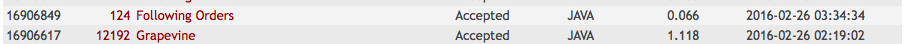
\includegraphics[width=\textwidth]{uvaResults}
%\newpage

%%%%%%% start Bank Cards %%%%%%%%%%%%%%%%%%%%%%%%%%%%%%%%%%%%%%%%%%

\section{UVA Problem 10937: Blackbeard}
\textbf{Background} \\
~\indent Blackbeard the Pirate has stashed up to 10 treasures on a tropical
island, and now he wishes to retrieve them.  He is being chased
by several authorities however, and so would like to retrieve his
treasure as quickly as possible. Blackbeard is no fool; when he hid
the treasures, he carefully drew a map of the island which contains
the position of each treasure and positions of all obstacles and hostile
natives that are present on the island. \\
\indent Given a map of an island and the point where he comes ashore,
help Blackbeard determine the least amount of time necessary for
him to collect his treasure. \\ \\
\textbf{Input} \\
~ \indent Input consists of a number of test cases. The  rst line of each test
case contains two integers $h$ and $w$ giving the height and width of
the map, respectively, in miles. For simplicity, each map is divided
into grid points that are a mile square. The next $h$ lines contain $w$
characters, each describing one square on the map. Each point on
the map is one of the following:
\begin{itemize}
    \item @ The landing point where Blackbeard comes ashore.
    \item $\sim$ Water. Blackbeard cannot travel over water while on the island.
    \item \# A large group of palm trees; these are too dense for Blackbeard to travel through
    \item $\cdot$ Sand, which he can easily travel over.
    \item $\ast$ A camp of angry natives.  Blackbeard must stay at least one square away or risk
    being captured by them which will terminate his quest. Note, this is one square in any of
    eight directions, including diagonals.
    \item ! A treasure. Blackbeard is a stubborn pirate and will not leave unless he
    collects all of them.
\end{itemize}
\indent Blackbeard can only travel in the four cardinal directions; that is, he cannot travel
diagonally. Blackbeard travels at a nice slow pace of one mile (or square) per hour, but he sure
can dig fast, because digging up a treasure incurs no time penalty whatsoever. \\
\indent The maximum dimension of the map is 50 by 50. The input ends with a case where both
$h$ and $w$ are 0. This case should not be processed. \\ \\
\textbf{Output} \\
~ \indent For each test case, simply print the least number of hours Blackbeard needs to
collect all his treasure and return to the landing point. If it is impossible to reach all
the treasures, print out `'-1'

%%%%%%% end Problem %%%%%%%%%%%%%%%%%%%%%%%%%%%%%%%%%%%%%%%%%%%%%%%

\newpage

%%%%%%% Mathematical Formulation %%%%%%%%%%%%%%%%%%%%%%%%%%%%%%%%%%
\subsection{Mathematical Formulation}
Given an input of the above described map with $n$ treasures and a starting position we will
determine whether or not all treasures are reachable, if so the distances between all of them
and the length of the shortest path to start at the starting point, visit every treasure, and
return to the start point.

%%%%%%% Algorithm %%%%%%%%%%%%%%%%%%%%%%%%%%%%%%%%%%%%%%%%%%%%%%%%%

\subsection{Solution}
Important Confusing Data Structures:
\begin{itemize}
    \item int \textbf{R, C, numTreasures} : ~ Stores (respectively), the max number rows and columns
     in the given map and the total number of treasures.
    \item char[R][C] \textbf{map} : ~ Stores the map provided from the input, then altered so that any
        un-crossable peice of land is represented as the symbol '\#' in $replaceCamps()$
    \item int[numTreasures+1][numTreasures+1] \textbf{dist} : ~ Stores the distnaces between two treasures
        (or the source). Built through calls to $bfs()$.
    \item int[numTreasures+1][2] \textbf{tresLoc} : ~ Stores the row and column coordinates of each
        treasure, $t_1\rightarrow(x_1,y_1), t_2\rightarrow(x_2,y_2), ..., t_n\rightarrow(x_n,y_n)$ at
        indexes $1..n$. Index 0 corresponds with the coordinates of the source.
    \item HashMap$\textless$Integer$\textgreater\textless$Integer$\textgreater$ \textbf{index} : ~
        Keeps track of the index of each treasure based off their [row][col] coordinates. The keys
        were (row$\cdot$\textbf{R}+col) and the value as the treasures index in the \textbf{dist} array.
        This is initialized and built in $locateTreasure()$ and used in $bfs()$.
    \item int[] \textbf{dr, dc} : ~ These arrays are \textbf{dr} $\gets$ \{-1,  0, 0, 1, 1, -1, -1,  1\}
        and \textbf{dr} $\gets$ \{ 0, -1, 1, 0, 1, -1,  1, -1\} which when put together will give you
        left, down, up, right, up/right, down/left, up/left, down/right. The whole arrays are used in the
        $replaceCamps()$ whereas, only the first 4 entries are used for the $bfs()$ since Blackbeard can
        only move in the 4 cardinal directions (not diagonally).
    \item HashMap$\textless$String$\textgreater\textless$Integer$\textgreater$ \textbf{mtsp} : ~ This is
        the hashmap which stores the intermediate values for the tsp $\therefore$ only seen in $tsp()$.
        Given $n$ total treasures each key will be some string i.e. n = 6, string = 10001003. We can break
        this up such that the first n+1 characters are either 0 or 1, (1 is the presence of that indexed
        treasure and 0 is the absence) and the first character (string.charAt(0)) is always 1 signifying
        we always have the source. Then the final character is a number $s,\ 1\leq s\leq n$, symbolizing
        that this number is the index of the treasure which we want to be last. Therefore putting all of
        them together gives us a subset where the source is always present followed by either 1's or 0's
        (if any intermeditate treasures) and finally the index of the last treasure in the subset.
\end{itemize}

The main functionality of this algorithm is to process the given map and put more constraints on it, then
construct a distance adjacency list using a breadth first search, essentially building a fully connected
graph, then finally running the Traveling Salesman Problem solution on this.

\begin{algorithm}[H]
\caption{Main}
\begin{algorithmic}
    \Procedure{main}{ }
        \While{true}
            \State $R, C \gets$ number of Rows and Columns respectively
            \If{R == C == 0}
                break;
            \EndIf
            \State Fill $map$ from input and count number of Treasures
            \State $numTreasures \gets$ number of Treasures on map
            \If{numTreasures == 0}
                \State \Call{Print}{-1}; continue;
            \EndIf
            \State \Call{replaceCamps}{ }  // see Algorithm 2
            \If{!locateTreasures()} // see Algorithm 3
                \State \Call{Print}{-1}; continue;
            \Else
                \State $boolean reachable \gets$ true
                \State $dist[][] \gets$ init
                \For{each treasure, t}
                    \If{!bfs($t_x$,$t_y$)}  // see Algorithm 4
                        \State $reachable \gets$ false; break;
                    \EndIf
                \EndFor
                \If{!reachable}
                    \State \Call{Print}{-1}; continue;
                \EndIf
            \EndIf
        \EndWhile
    \EndProcedure
\end{algorithmic}
\end{algorithm}

When we are altering the map[ ][ ], what we want to do is to replace all instances of water and
angry native camps with the same symbol for trees. In addition, we are also ensuring that we
change the surrounding area of the camps as described in the problem description.

\begin{algorithm}[H]
\caption{Alter the Map}
\begin{algorithmic}
    \Procedure{replaceCamps}{ }
        \For{row $\in$ 0..R, col $\in$ 0..C}
            \State $char c \gets$ map[row][col]
            \If{c == '$\sim$'}
                $map[row][col] \gets$ '\#';
            \ElsIf{c == '$\ast$'}
                \State $map[row][col] \gets$ '\#';
                \For{i $\in$ 0..dc.length}
                    \State $int\ rPrime, cPrime \gets$ row + dr[i], col + dc[i]
                    \If{(rPrime and cPrime in bounds) and (not a camp)}
                        \State $map[rPrime][cPrime] \gets$ '\#'
                    \EndIf
                \EndFor
            \EndIf
        \EndFor
    \EndProcedure
\end{algorithmic}
\end{algorithm}

Once we have Altered this we need to initialize index and tresLoc and ensure that we still
have all of our treasures and start point (these could have been erased in the $replaceCamps()$
method). We will return false if either of these have been altered.

\begin{algorithm}[H]
\caption{Build Support for dist array and ensure treasures preserved}
\begin{algorithmic}
    \Procedure{locateTreasures}{ }
        \State $index, tresLoc \gets$ init, boolean start = false, count = 0
        \For{row $\in$ 0..R, col $\in$ 0..C}
            \If{map[row][col] == '@'}
                \State $start \gets$ true
                \State $tresLoc[0][0,1] \gets$ row, col
            \ElsIf{map[row][col] == '!'}
                \State index.\Call{put}{row*R+col, ++count}
                \State $tresLoc[count][0,1] \gets$ row, col
            \EndIf
        \EndFor
        \State return start \&\& (count==numTreasures)
    \EndProcedure
\end{algorithmic}
\end{algorithm}

Once we have built our adjacency distance array, we can perform the Travelling Salesman Problem
solution. We do this using our HashMap mtsp  (see explanation of data structure above for details).

\begin{algorithm}[H]
\caption{Traveling Salesman Problem, determine cost of minimum path}
\begin{algorithmic}
    \Procedure{tsp}{ }
        \State $mtsp \gets$ init; int length = (2 \textless\textless (dist.length-2));
        \State // build up the dp hashmap
        \For{$i \in [length,(length \textless\textless 1)]$}
            \State $char[ ]\ bitRep \gets$ Binary representation of i
            \For{$c \in [1,BitRep.length]$}
                \If{bitRep[c] == '1'}
                    \State $bestVal \gets$ MAX\_VALUE;
                    \For{$k \in [1,bitRep.length]$}
                        \If{bitRep[k] == '1'}
                            \State $val \gets$ mtsp.get(cToString(bitRep,k)) + dist[k][c]
                            \If{val \textless bestVal}
                                bestVal = val
                            \EndIf
                        \EndIf
                    \EndFor
                    \State mtsp.put(cToString(bitRep, c), bestVal);
                \EndIf
            \EndFor
        \EndFor
        \State // determine the best option on how to return to the source
        \State $lastLevel \gets$ full bit representation (all 1's); $best \gets$ MAX\_VALUE
        \For{$i \in [1,lastLevel.length]$}
            \State $val \gets$ mtsp.get(cToString(lastLevel, i)) + dist[i][0];
            \If{val \textless best}
                $best \gets$ val
            \EndIf
        \EndFor
        \State Print best;
    \EndProcedure
\end{algorithmic}
\end{algorithm}

%%%%%%% Correctness %%%%%%%%%%%%%%%%%%%%%%%%%%%%%%%%%%%%%%%%%%%%%%%

\subsection{Correctness}
%%%%%%% PROPOSITION 1 %%%%%%%%%%%%%%%
\begin{proposition}
~ \\ \indent This is clearly a TSP problem for which we need a fully connected graph G
and we can each node is either a treasure or the source
\end{proposition}

\begin{proof}
~ \\ \indent Using the fact that 
\end{proof}


%%%%%%% Analysis %%%%%%%%%%%%%%%%%%%%%%%%%%%%%%%%%%%%%%%%%%%%%%%%%%
\subsection{Analysis}
For the following analysis, we will say that the map that we are given is of dimensions
$RxC$ which contains N treasures and 1 source. It should be noted that N is (in the typical case)
much smaller than $R\cdot C$.


%%%%%%% PROPOSITION 1 %%%%%%%%%%%%%%%
\begin{proposition}
\label{numq}
The \underline{space complexity} of this algorithm is \textbf{O(R$\cdot$C+N$\cdot$2$^N$)}
\end{proposition}

\begin{proof}
~ \\ \indent This is due to the fact that all of our data is stored in data structures:
\begin{itemize}
    \item \underline{map}: Stores the map $\implies R\cdot C$
    \item \underline{tresLoc}: Stores the location of each treasure on the map $\implies 2\cdot (N+1)$
    \item \underline{dist}: The adjacency matrix for all treasures and the source $\implies (N+1)^2$
    \item \underline{index}: Indicies of the treasures in the distance array based off of
            their coordinates in the map $\implies N$
    \item \underline{mtsp}: Stores all of the sub-problem solutions to tsp $\implies N\cdot 2^N$
\end{itemize}
Summing these all together we get $(R\cdot C) + (2\cdot(N+1)^3) + (N) + (N\cdot2^N)$
\begin{center}
    Giving us a space complexity of \textbf{O(R$\cdot$C+N$\cdot$2$^N$)}
\end{center}
\end{proof}

%%%%%%% PROPOSITION 2 %%%%%%%%%%%%%%%
\begin{proposition}
\label{numq}
The \underline{time complexity} of this algorithm is \textbf{O(N$\cdot$R$\cdot$C+N$\cdot$2$^N$)}
\end{proposition}

\begin{proof}
This is the case because our algorithm performs the following actions: build the map ($R\cdot C$);
alter the map ($R\cdot C$); locate the treasures ($R\cdot C$); perform a bfs witch each treasure as
the source ($N\cdot R\cdot C$); perform traveling salesman problem using all of the treasures as
nodes ($N\cdot 2^N$).  When we sum this together we get $2\cdot(R\cdot C) + (N\cdot R\cdot C) +
(N\cdot 2^N)$
\begin{center}
    Giving us a time complexity of \textbf{O(N$\cdot$R$\cdot$C+N$\cdot$2$^N$)}
\end{center}
\end{proof}

%%%%%%% Example %%%%%%%%%%%%%%%%%%%%%%%%%%%%%%%%%%%%%%%%%%%%%%%%%%%

\subsection{An Example}
We read in the input in our map[5][5] and then convert it to our uniform form:
\[
map =
\begin{bmatrix}
 .& !& .& \#& \sim         \\
 \sim& .& .& .& \sim       \\
 \ast& .& \#& .& @         \\
 \sim& \#& \#& .& \sim     \\
 \sim& \sim& \sim& !& \sim \\
\end{bmatrix}
\rightarrow
\begin{bmatrix}
.&   !&  .& \#& \# \\
\#& \#&  .&  .& \# \\
\#& \#& \#&  .&  @ \\
\#& \#& \#&  .& \# \\
\#& \#& \#&  !& \# \\
\end{bmatrix}
\]
We see that both treasures and the source are still there so we proceed with
computing a bfs with each source and two treasures as the source producing:
\[
source =
\begin{bmatrix}
6&   \textbf{5}&  4& \#& \# \\
\#& \#&  3&  2& \# \\
\#& \#& \#&  1&  \textbf{0} \\
\#& \#& \#&  2& \# \\
\#& \#& \#&  \textbf{3}& \# \\
\end{bmatrix}
,\ t_1 =
\begin{bmatrix}
1&   \textbf{0}&  1& \#& \# \\
\#& \#&  2&  3& \# \\
\#& \#& \#&  4&  \textbf{5} \\
\#& \#& \#&  5& \# \\
\#& \#& \#&  \textbf{6}& \# \\
\end{bmatrix}
,\ t_2 =
\begin{bmatrix}
7&   \textbf{6}&  5& \#& \# \\
\#& \#&  4&  3& \# \\
\#& \#& \#&  2&  \textbf{3} \\
\#& \#& \#&  1& \# \\
\#& \#& \#&  \textbf{0}& \# \\
\end{bmatrix}
\]
Then from these we get the distance array:
\[
dist =
\begin{bmatrix}
0 & 5 & 3 \\
5 & 0 & 6 \\
3 & 6 & 0 \\
\end{bmatrix}
\]
Therefore we can now begin our Traveling salesman problem, we start with 101 and can therefore
start building up our DP solution.
\[
101 \implies \{s,t_2\} =
\begin{cases}
1002
\end{cases}
= dist[s][t_2] = dist[0][2] = 3
\]
\[
110 \implies \{s,t_1\} =
\begin{cases}
1001
\end{cases}
= dist[s][t_1] = dist[0][1] = 5
\]
\[
111 \implies \{s,t_2,t_1\} =
\begin{cases}
1011 \\
1102
\end{cases}
=
\begin{cases}
101 + dist[t_2][t_1] = 1002 + dist[1][2] = 3 + 6 = 9 \\
110 + dist[t_1][t_2] = 1001 + dist[2][1] = 5 + 6 = 11
\end{cases}
\]
\[
best \implies \{s,t_2,t_1,s\} =
\begin{cases}
1011 + d[t_1][0] = 9  + 5 = 14\\
1102 + d[t_2][0] = 11 + 3 = 14
\end{cases}
\]
Therefore we have the least cost as 14.

%%%%%%% end Bank Cards %%%%%%%%%%%%%%%%%%%%%%%%%%%%%%%%%%%%%%%%%%%


%%%%%%% end Solution %%%%%%%%%%%%%%%%%%%%%%%%%%%%%%%%%%%%%%%%%%%%%%

\end{document}